% Unofficial UofT Poster template.
% A fork of the UMich template https://www.overleaf.com/latex/templates/university-of-michigan-umich-poster-template/xpnqzzxwbjzc
% which is fork of the MSU template https://www.overleaf.com/latex/templates/an-unofficial-poster-template-for-michigan-state-university/wnymbgpxnnwd
% which is a fork of https://www.overleaf.com/latex/templates/an-unofficial-poster-template-for-new-york-university/krgqtqmzdqhg
% which is a fork of https://github.com/anishathalye/gemini
% also refer to https://github.com/k4rtik/uchicago-poster

\documentclass[final]{beamer}

% ====================
% Packages
% ====================

\usepackage[T1]{fontenc}
\usepackage[utf8]{luainputenc}
\usepackage{lmodern}
\usepackage[size=custom, width=125,height=93, scale=1.2]{beamerposter}
\usetheme{gemini}
\usecolortheme{uoft}
\usepackage{graphicx}
\usepackage{booktabs}
\usepackage{tikz}
\usepackage{pgfplots}
\pgfplotsset{compat=1.14}
\usepackage{anyfontsize}
\usepackage[font=small,textfont=it,skip=1pt,labelfont=bf]{caption}
\usepackage{datetime}

% ====================
% Lengths
% ====================

% If you have N columns, choose \sepwidth and \colwidth such that
% (N+1)*\sepwidth + N*\colwidth = \paperwidth
\newlength{\sepwidth}
\newlength{\colwidth}
\setlength{\sepwidth}{0.025\paperwidth}
\setlength{\colwidth}{0.3\paperwidth}


\newcommand{\separatorcolumn}{\begin{column}{\sepwidth}\end{column}}

\setlength{\parskip}{1em}
% ====================
% Title
% ====================

\title{Analyzing Patterns of Computational Similarity between Kinase Ligands}

\author{Jack Ringer}

\institute[shortinst]{University of New Mexico\\8/4/2025}

% ====================
% Footer (optional)
% ====================

\footercontent{
  \href{https://github.com/Jack-42/ligandActivityAnalysis}{GitHub: https://github.com/Jack-42/ligandActivityAnalysis} \hfill
CFDE Summer Internship at UNM, 2025 \hfill
{johnjack0987@gmail.com}}
% (can be left out to remove footer)

% ====================
% Logo (optional)
% ====================

% use this to include logos on the left and/or right side of the header:
% Left: institution
 \logoright{
\includegraphics[height=8cm]{logos/unm_hsc.jpg}}
% Right: funding agencies and other affilations 
%\logoright{\includegraphics[height=7cm]{logos/NSF.eps}}
% ====================
% Body
% ====================

\begin{document}


\begin{frame}[t]
\begin{columns}[t]
\separatorcolumn

\begin{column}{\colwidth}

  \begin{block}{Background and Overview}
  \heading{Background}
   \small

 There are 8 major groups within the human kinome, which include: AGC, CAMK, CK1, CMGC, STE, TK, TKL, Other, as well as 13 atypical families~\cite{eid_turk_volkamer_rippmann_fulle_2017, manning_2002}. Aside from the ``Atypical'' and ``Other'' groups, these group classifications are generally based on sequence similarity, evolutionary conservation, and known functions. 

\begin{figure}[H]
    \centering
    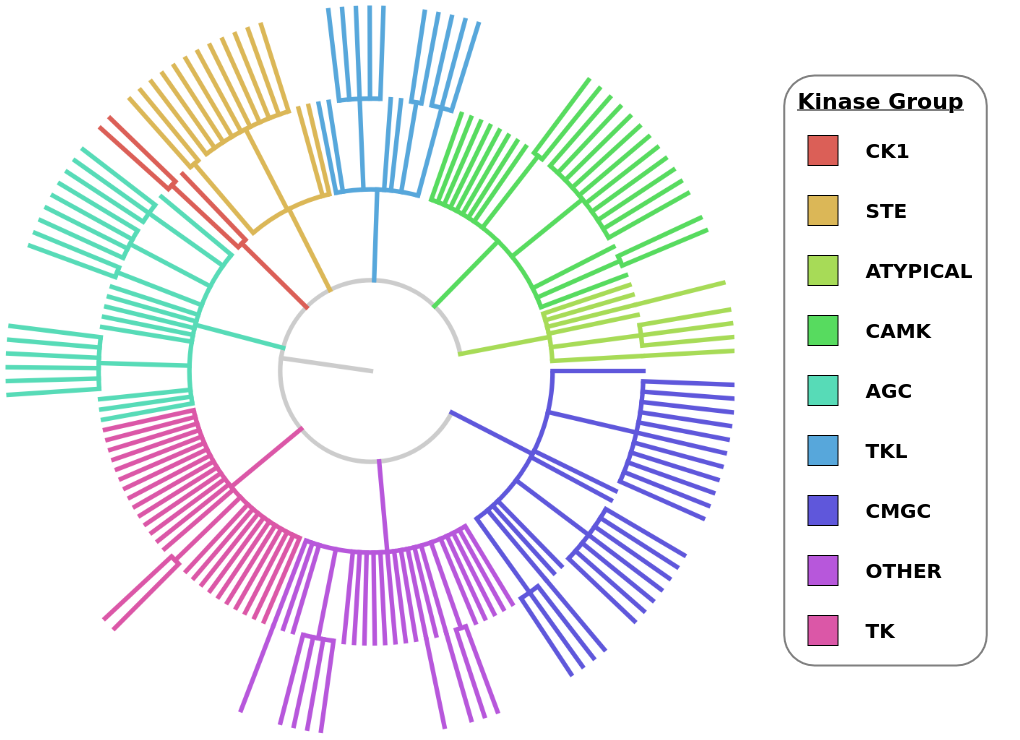
\includegraphics[width=0.5\textwidth]{../figures/protein_family_tree.png}
    \caption{Phylogenetic Tree of the human kinome showing major groups as well as families and subfamilies. Generated using ETE4 with data from ChEMBL~\cite{chembl_db_2023}.}
    \label{fig:fam_tree}
\end{figure}

The similarity property principle (SPP), has been enormously influential in the realm of medicinal chemistry~\cite{maggiora_vogt_stumpfe_bajorath_2013}. According to the SPP, structurally-similar compounds often exhibit similar properties (including biological activity). 

This work investigates whether ligands which are active within a particular protein kinase group are more similar to one another than protein kinase ligands generally. 
    \heading{Why is this important?}
    \begin{itemize}
        \item Relevant to drug discovery research
        \item If there is a relationship between protein kinase group and ligand similarity, then it may be informative to look at the ligands of related protein kinases (i.e., those belonging to the same group)
    \end{itemize}

  \end{block}

  \begin{block}{Dataset and Methodology}
    \small
    The set of active ligands and their relationship to specific human protein kinases was determined using data from single protein target binding assays in the ChEMBL database~\cite{chembl_db_2023}. 
    \begin{itemize}
        \item Assay/ligand selection based on Pharos~\cite{pharos_2022}
        \item Remove assays where target was a variant/mutant
        \item Filtered out PAINS compounds~\cite{baell_holloway_2010}
        \item Molecular weight of ligand must fall between [200, 900] Da
    \end{itemize}

    The criteria above resulted in a dataset with the folllowing properties:

    \begin{table}[!ht]
    \centering
    \small
    \begin{tabular}{l|l}
        \hline
        \textbf{Variable} & \textbf{Value} \\ \hline
        N. Protein Targets & 423 \\ \hline
        N. Assays & 73,487 \\ \hline
        N. Active Samples & 38,622 \\ \hline
        N. Unique Ligands & 9,995 \\ \hline
    \end{tabular}
    \end{table}

    Ligands are considered active within a protein kinase group if they were identified as an active within an assay targeting a protein belonging to the group. 

    After determining the set of ligands and their group relationship(s), Morgan fingerprints were computed using RDKit. Tanimoto similarity coefficients were then computed between these 2D fingerprints. Figure~\ref{ligand_sim} shows the 2D structures of some ligand pairs and their similarity values.
\begin{figure}
    \centering
    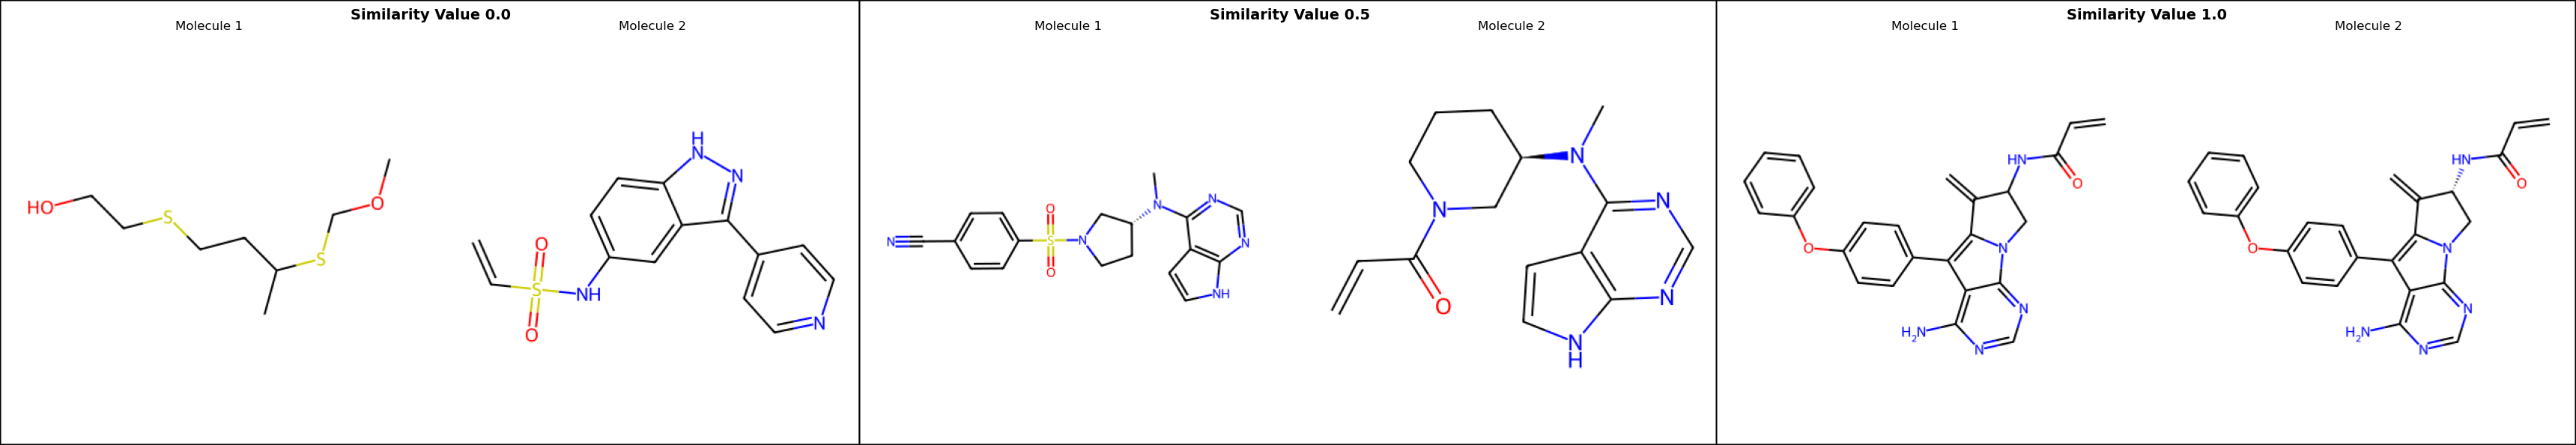
\includegraphics[width=\textwidth]{../figures/ligand_sim.png}
    \caption{Pairs of protein kinase ligands and their Tanimoto similarity values (0, 0.5, 1).}
    \label{ligand_sim}
\end{figure}

 

  \end{block}
\end{column}

\separatorcolumn

\begin{column}{\colwidth}

  \begin{block}{Results}
    \small
    Figure~\ref{violin_plot} provides distributions for the ${N\choose 2}$ similarity values per group ($N$ = number of ligands), as well as the ${9,995 \choose 2} = 49,945,015$ similarity values calcualted for all protein kinase ligands in the dataset. Table~\ref{results_table} provides additional statistics for each group and results from a Mann-Whitney U test (MWUT).
    \begin{figure}
        \centering
        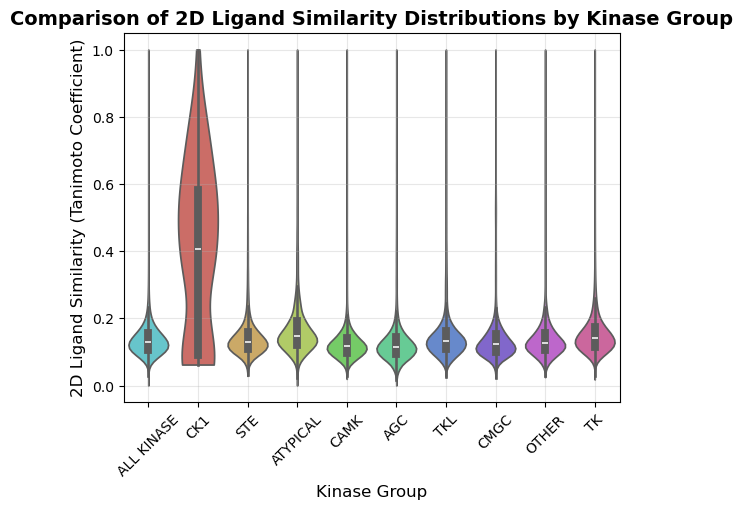
\includegraphics[width=0.75\textwidth]{../figures/violin_plot.png}
        \caption{Comparison of 2D structural similarity distributions by protein kinase group}
        \label{violin_plot}
    \end{figure}
    
    \begin{table}[!ht]
    \centering
    \footnotesize
    \begin{tabular}{l|l|l|l|l|l}
        \hline
        \textbf{Kinase Group} & \textbf{N. Targets} & \textbf{N. Ligands} & \textbf{Group Median} &\textbf{Comparison Median} & \textbf{MWUT p-value} \\ \hline
        CK1 & 10 & 13 & 0.407 & 0.129 & $3.10 \times 10^{-11}$ \\ \hline
        STE & 45 & 425 & 0.131 & 0.129 & $2.48 \times 10^{-169}$ \\ \hline
        ATYPICAL & 15 & 357 & 0.149 & 0.129 & $< 5 \times 10^{-324}$ \\ \hline
        CAMK & 65 & 597 & 0.117 & 0.130 & $1.0$ \\ \hline
        AGC & 59 & 809 & 0.116 & 0.131 & $1.0$ \\ \hline
        TKL & 37 & 810 & 0.133 & 0.129 & $< 5 \times 10^{-324}$ \\ \hline
        CMGC & 58 & 1275 & 0.122 & 0.130 & $1.0$ \\ \hline
        OTHER & 56 & 727 & 0.127 & 0.129 & $1.0$ \\ \hline
        TK & 80 & 5347 & 0.140 & 0.121 & $< 5 \times 10^{-324}$ \\ \hline
    \end{tabular}
    \caption{Table showing comparisons of targets, ligands, and ligand similarity distributions per protein kinase group. Shown p-values are calculated (with Bonferroni correction) from a MWUT where the alternative hypothesis is that the similarity values within the group are stochastically greater than the distribution of all other similarity values.}\label{results_table}
    \end{table}
    Figure~\ref{enrichment_plot} below shows the enrichment values observed for different protein kinase groups, where enrichment is defined as:
    \begin{equation*}
        \footnotesize
        \frac{P(\text{two ligands active within group} \; | \; \text{similarity} > \text{threshold})}{P(\text{two ligands active within group})}
    \end{equation*}
    \begin{figure}
        \centering
        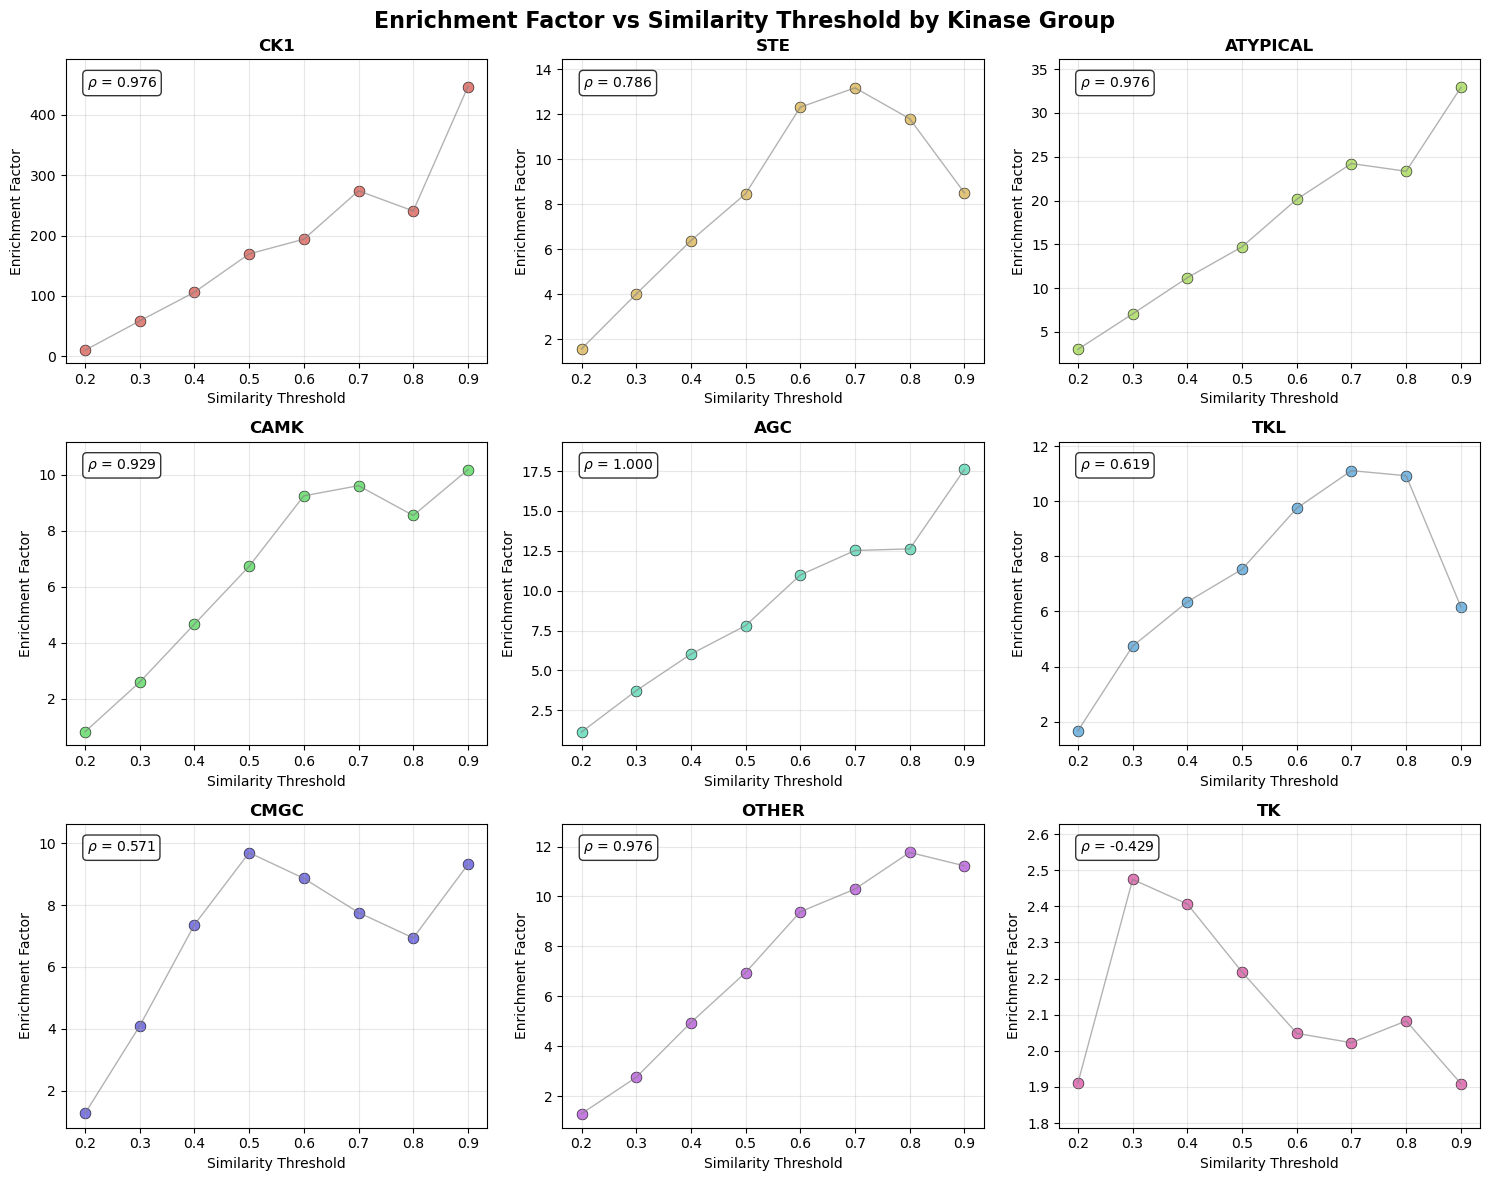
\includegraphics[width=0.85\textwidth]{../figures/enrichment_factor_by_group.png}
        \caption{Plot of enrichment values by protein kinase group.}
        \label{enrichment_plot}
    \end{figure}

  \end{block}

\end{column}

\separatorcolumn

\begin{column}{\colwidth} 
  \begin{block}{Discussion}
    \small
    \heading{Limitations}
    \begin{itemize}
        \item Not all protein targets are equally well-studied (see Figure~\ref{assay_vs_ligand_plot})
        \item Only considered Morgan fingerprints + Tanimoto coefficients when measuring ``similarity'' of ligands
        \item Methodology does not directly account for differences in assay conditions, or the fact that even single proteins can have multiple binding sites
        \item Data gathered from ChEMBL may not reflect global trends
    \end{itemize}

    \begin{figure}
        \centering
        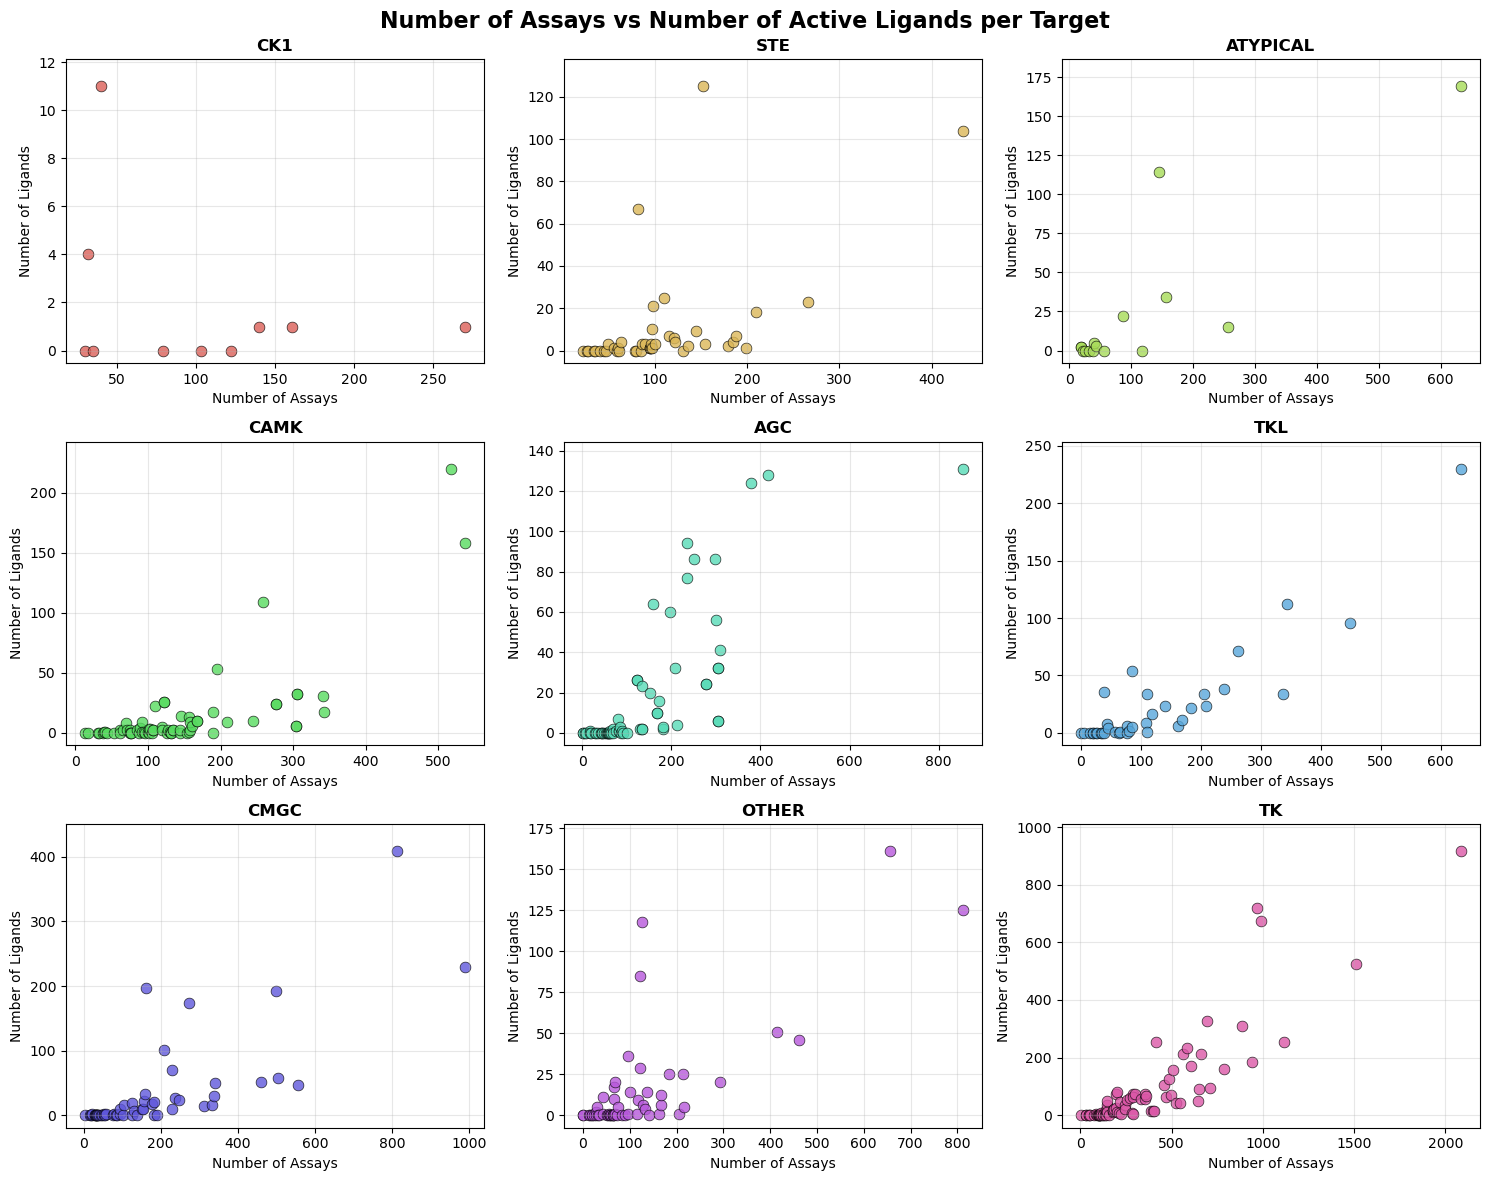
\includegraphics[width=0.85\textwidth]{../figures/assay_vs_ligand.png}
        \caption{Scatter plots showing the number of assays (x-axis) and ligands (y-axis) for each protein belonging to each protein kinase group.}
        \label{assay_vs_ligand_plot}
    \end{figure}

    \heading{Conclusions}
      \small
      Overall, this study found no clear relationship between 2D ligand similarity and protein kinase group activity. Although significant differences were observed for the CK1 group, given the limitations outlined above further study is necessary before accepting these results. 
  \end{block}

  \begin{block}{Acknowledgements}
  \small{
    Much thanks to my advisor Dr.~Vincent Metzger for his guidance and input over the course of this project. I'd also like to thank Dr.~Jeremy Yang, Dr.~Cristian Bologa, and Dr.~Praveen Kumar for their feedback during weekly meetings over the course of the internship. Finally, I'd like to thank the   authors of ChEMBL DB~\cite{chembl_db_2023}.}
  \end{block}

  \begin{block}{References}
    \tiny{\bibliographystyle{plain}\bibliography{poster}}
  \end{block}

\end{column}

\separatorcolumn
\end{columns}
\end{frame}

\end{document}
